\documentclass[aps,prfluids,reprint,onecolumn,amsmath,amssymb,nofootinbib,floatfix]{revtex4-2}

\usepackage{graphicx}
\usepackage{amsmath,amssymb}
\usepackage{booktabs}
\usepackage{xcolor}
\usepackage{hyperref}
\usepackage{enumitem}

\newcommand{\code}[1]{\texttt{\small #1}}
\setlist[itemize]{itemsep=1pt, topsep=3pt, parsep=0pt}

\newcommand{\TabHeadSizes}{%
\begin{tabular}{rrrrrr}
\toprule
$N$ & bits/axis & blocks & \multicolumn{3}{c}{cells per block}\\
\cmidrule(l){4-6}
 & $N/2$ & $2^{N/2}\times2^{N/2}$ & $L=9$ & $L=10$ & $L=11$\\
\midrule
4 & 2 & $4\times4$ & 128 & 256 & 512\\
6 & 3 & $8\times8$ & 64 & 128 & 256\\
8 & 4 & $16\times16$ & 32 & 64 & 128\\
10 & 5 & $32\times32$ & 16 & 32 & 64\\
12 & 6 & $64\times64$ & 8 & 16 & 32\\
\bottomrule
\end{tabular}}

\newcommand{\TabRateDistortion}{%
\textbf{$L=8$ ($256^2$)}\\[2pt]
\begin{tabular}{rrrrrr}
\toprule
$N$ & $\chi$ & $\rho$ & head\,\% & $L_2$ (evolution) & $L_2$ (representation)\\
\midrule
0 & 8 & 0.0221 & -- & $7.96\times10^{-1}$ & $1.62\times10^{-1}$\\
0 & 12 & 0.0436 & -- & $3.35\times10^{-1}$ & $6.92\times10^{-2}$\\
0 & 16 & 0.0729 & -- & $1.22\times10^{-1}$ & $2.93\times10^{-2}$\\
0 & 24 & 0.1393 & -- & $2.64\times10^{-2}$ & $7.30\times10^{-3}$\\
0 & 32 & 0.2291 & -- & $3.57\times10^{-3}$ & $1.41\times10^{-3}$\\
4 & 8 & 0.0208 & 9 & $7.79\times10^{-1}$ & $1.62\times10^{-1}$\\
4 & 12 & 0.0423 & 7 & $3.22\times10^{-1}$ & $6.92\times10^{-2}$\\
4 & 16 & 0.0716 & 5 & $1.24\times10^{-1}$ & $2.93\times10^{-2}$\\
4 & 24 & 0.1380 & 3 & $2.66\times10^{-2}$ & $7.30\times10^{-3}$\\
4 & 32 & 0.2278 & 2 & $3.57\times10^{-3}$ & $1.41\times10^{-3}$\\
6 & 8 & 0.0228 & 34 & $3.44\times10^{-1}$ & $6.79\times10^{-2}$\\
6 & 12 & 0.0423 & 28 & $1.65\times10^{-1}$ & $2.98\times10^{-2}$\\
6 & 16 & 0.0677 & 23 & $6.76\times10^{-2}$ & $1.54\times10^{-2}$\\
6 & 24 & 0.1282 & 18 & $1.38\times10^{-2}$ & $4.34\times10^{-3}$\\
6 & 32 & 0.2083 & 15 & $3.58\times10^{-3}$ & $1.41\times10^{-3}$\\
8 & 8 & 0.0423 & 74 & $6.40\times10^{-2}$ & $1.57\times10^{-2}$\\
8 & 12 & 0.0687 & 68 & $1.39\times10^{-2}$ & $4.38\times10^{-3}$\\
8 & 16 & 0.0989 & 63 & $3.63\times10^{-3}$ & $1.59\times10^{-3}$\\
8 & 24 & 0.1634 & 57 & $5.21\times10^{-4}$ & $2.73\times10^{-4}$\\
8 & 32 & 0.2396 & 52 & $9.85\times10^{-5}$ & $5.14\times10^{-5}$\\
10 & 4 & 0.0648 & 97 & $1.30\times10^{-1}$ & $2.15\times10^{-2}$\\
10 & 6 & 0.0981 & 96 & $1.09\times10^{-2}$ & $4.78\times10^{-3}$\\
10 & 8 & 0.1321 & 95 & $5.32\times10^{-3}$ & $2.08\times10^{-3}$\\
10 & 12 & 0.2005 & 94 & $6.41\times10^{-4}$ & $3.46\times10^{-4}$\\
10 & 16 & 0.2708 & 92 & $1.00\times10^{-4}$ & $6.87\times10^{-5}$\\
\bottomrule
\end{tabular}
\vspace{6pt}
\textbf{$L=9$ ($512^2$)}\\[2pt]
\begin{tabular}{rrrrrr}
\toprule
$N$ & $\chi$ & $\rho$ & head\,\% & $L_2$ (evolution) & $L_2$ (representation)\\
\midrule
0 & 12 & 0.0131 & -- & $7.23\times10^{-1}$ & $1.36\times10^{-1}$\\
0 & 16 & 0.0221 & -- & $4.20\times10^{-1}$ & $7.39\times10^{-2}$\\
0 & 24 & 0.0436 & -- & $1.50\times10^{-1}$ & $2.33\times10^{-2}$\\
0 & 32 & 0.0729 & -- & $3.95\times10^{-2}$ & $6.65\times10^{-3}$\\
8 & 12 & 0.0194 & 61 & $1.35\times10^{-1}$ & $1.85\times10^{-2}$\\
8 & 16 & 0.0286 & 55 & $6.20\times10^{-2}$ & $9.17\times10^{-3}$\\
8 & 24 & 0.0496 & 47 & $1.30\times10^{-2}$ & $2.30\times10^{-3}$\\
8 & 32 & 0.0755 & 41 & $3.13\times10^{-3}$ & $7.48\times10^{-4}$\\
10 & 12 & 0.0523 & 90 & $1.30\times10^{-2}$ & $1.93\times10^{-3}$\\
10 & 16 & 0.0716 & 87 & $2.69\times10^{-3}$ & $7.28\times10^{-4}$\\
10 & 24 & 0.1112 & 84 & $3.47\times10^{-4}$ & $1.19\times10^{-4}$\\
10 & 32 & 0.1536 & 81 & $5.32\times10^{-5}$ & $1.98\times10^{-5}$\\
\bottomrule
\end{tabular}
\vspace{6pt}
\textbf{$L=10$ ($1024^2$)}\\[2pt]
\begin{tabular}{rrrrrr}
\toprule
$N$ & $\chi$ & $\rho$ & head\,\% & $L_2$ (evolution) & $L_2$ (representation)\\
\midrule
0 & 16 & 0.0065 & -- & $8.28\times10^{-1}$ & $1.15\times10^{-1}$\\
0 & 24 & 0.0131 & -- & $3.96\times10^{-1}$ & $4.51\times10^{-2}$\\
0 & 32 & 0.0221 & -- & $1.70\times10^{-1}$ & $1.73\times10^{-2}$\\
0 & 48 & 0.0436 & -- & $3.54\times10^{-2}$ & $3.55\times10^{-3}$\\
0 & 64 & 0.0729 & -- & $5.46\times10^{-3}$ & $6.41\times10^{-4}$\\
8 & 16 & 0.0081 & 48 & $2.62\times10^{-1}$ & $2.54\times10^{-2}$\\
8 & 24 & 0.0146 & 40 & $1.03\times10^{-1}$ & $9.67\times10^{-3}$\\
8 & 32 & 0.0228 & 34 & $4.41\times10^{-2}$ & $4.10\times10^{-3}$\\
8 & 48 & 0.0423 & 28 & $7.60\times10^{-3}$ & $8.50\times10^{-4}$\\
8 & 64 & 0.0677 & 23 & $1.56\times10^{-3}$ & $2.16\times10^{-4}$\\
10 & 16 & 0.0189 & 83 & $5.19\times10^{-2}$ & $3.77\times10^{-3}$\\
10 & 24 & 0.0300 & 78 & $1.02\times10^{-2}$ & $9.06\times10^{-4}$\\
10 & 32 & 0.0423 & 74 & $2.03\times10^{-3}$ & $2.66\times10^{-4}$\\
10 & 48 & 0.0687 & 68 & $1.62\times10^{-4}$ & $3.19\times10^{-5}$\\
10 & 64 & 0.0990 & 63 & $1.92\times10^{-5}$ & $4.68\times10^{-6}$\\
12 & 16 & 0.0648 & 96 & $2.27\times10^{-3}$ & $3.20\times10^{-4}$\\
12 & 24 & 0.0981 & 96 & $1.80\times10^{-4}$ & $3.71\times10^{-5}$\\
12 & 32 & 0.1322 & 95 & $2.26\times10^{-5}$ & $6.34\times10^{-6}$\\
12 & 48 & 0.2005 & 94 & $6.80\times10^{-7}$ & $2.46\times10^{-7}$\\
12 & 64 & 0.2708 & 92 & $3.26\times10^{-8}$ & $1.06\times10^{-8}$\\
\bottomrule
\end{tabular}
\vspace{6pt}
\textbf{$L=11$ ($2048^2$)}\\[2pt]
\begin{tabular}{rrrrrr}
\toprule
$N$ & $\chi$ & $\rho$ & head\,\% & $L_2$ (evolution) & $L_2$ (representation)\\
\midrule
0 & 24 & 0.0038 & -- & $9.29\times10^{-1}$ & $6.50\times10^{-2}$\\
0 & 32 & 0.0065 & -- & $5.31\times10^{-1}$ & $2.94\times10^{-2}$\\
0 & 48 & 0.0131 & -- & $1.60\times10^{-1}$ & $7.36\times10^{-3}$\\
0 & 64 & 0.0221 & -- & $4.40\times10^{-2}$ & $1.82\times10^{-3}$\\
10 & 24 & 0.0080 & 73 & $8.84\times10^{-2}$ & $3.64\times10^{-3}$\\
10 & 32 & 0.0116 & 68 & $3.13\times10^{-2}$ & $1.44\times10^{-3}$\\
10 & 48 & 0.0194 & 61 & $4.77\times10^{-3}$ & $2.71\times10^{-4}$\\
10 & 64 & 0.0286 & 55 & $8.72\times10^{-4}$ & $6.47\times10^{-5}$\\
12 & 24 & 0.0251 & 93 & $8.99\times10^{-3}$ & $3.73\times10^{-4}$\\
12 & 32 & 0.0340 & 92 & $1.32\times10^{-3}$ & $1.04\times10^{-4}$\\
12 & 48 & 0.0523 & 90 & $6.89\times10^{-5}$ & $9.70\times10^{-6}$\\
12 & 64 & 0.0716 & 87 & $6.26\times10^{-6}$ & $1.08\times10^{-6}$\\
\bottomrule
\end{tabular}
\vspace{6pt}}

\newcommand{\TabBudgetSaving}{%
\begin{tabular}{rrrrr}
\toprule
target $L_2$ & $L=8$ & $L=9$ & $L=10$ & $L=11$\\
\midrule
$1\times10^{-1}$ & 1.4 ($N{=}6$) & 2.3 ($N{=}8$) & 1.9 ($N{=}8$) & --\\
$6\times10^{-2}$ & 2.3 ($N{=}8$) & 2.1 ($N{=}8$) & 1.8 ($N{=}8$) & 2.1 ($N{=}10$)\\
$3\times10^{-2}$ & 2.5 ($N{=}8$) & -- & 2.1 ($N{=}10$) & --\\
$1\times10^{-2}$ & 2.4 ($N{=}8$) & -- & 2.1 ($N{=}10$) & --\\
$3\times10^{-3}$ & -- & -- & -- & --\\
\bottomrule
\end{tabular}}

\newcommand{\TabCost}{%
\begin{tabular}{rrrrr}
\toprule
$L$ & $N$ & $\chi$ & $\rho$ & ms/step\\
\midrule
8 & 0 & 32 & 0.2291 & 846\\
8 & 4 & 32 & 0.2278 & 920\\
8 & 6 & 32 & 0.2083 & 822\\
8 & 8 & 32 & 0.2396 & 535\\
9 & 0 & 32 & 0.0729 & 1507\\
9 & 8 & 32 & 0.0755 & 1419\\
9 & 10 & 32 & 0.1536 & 1518\\
10 & 0 & 32 & 0.0221 & 818\\
10 & 8 & 32 & 0.0228 & 940\\
10 & 10 & 32 & 0.0423 & 1068\\
10 & 12 & 32 & 0.1322 & 1989\\
11 & 0 & 32 & 0.0065 & 2257\\
11 & 10 & 32 & 0.0116 & 3348\\
11 & 12 & 32 & 0.0340 & 3596\\
\bottomrule
\end{tabular}}

\newcommand{\TabDNS}{%
\begin{tabular}{rrrrrr}
\toprule
$N$ & $\chi$ & $\rho$ & head\,\% & $L_2$ (evolution) & $L_2$ (representation)\\
\midrule
0 & 16 & 0.0221 & -- & $3.06\times10^{-1}$ & $5.94\times10^{-2}$\\
0 & 24 & 0.0436 & -- & $1.82\times10^{-1}$ & $2.97\times10^{-2}$\\
0 & 32 & 0.0729 & -- & $1.25\times10^{-1}$ & $1.37\times10^{-2}$\\
0 & 48 & 0.1393 & -- & $6.61\times10^{-2}$ & $5.03\times10^{-3}$\\
8 & 16 & 0.0286 & 55 & $1.51\times10^{-1}$ & $1.29\times10^{-2}$\\
8 & 24 & 0.0496 & 47 & $8.60\times10^{-2}$ & $6.46\times10^{-3}$\\
8 & 32 & 0.0755 & 41 & $8.44\times10^{-2}$ & $3.83\times10^{-3}$\\
8 & 48 & 0.1341 & 35 & $3.40\times10^{-2}$ & $1.85\times10^{-3}$\\
10 & 16 & 0.0716 & 87 & $7.00\times10^{-2}$ & $2.62\times10^{-3}$\\
10 & 24 & 0.1112 & 84 & $1.34\times10^{-1}$ & $1.26\times10^{-3}$\\
10 & 32 & 0.1536 & 81 & $2.68\times10^{-2}$ & $7.22\times10^{-4}$\\
10 & 48 & 0.2396 & 78 & $1.84\times10^{-3}$ & $3.26\times10^{-4}$\\
12 & 16 & 0.2552 & 98 & $9.06\times10^{-2}$ & $3.89\times10^{-4}$\\
12 & 24 & 0.3836 & 98 & $4.47\times10^{-4}$ & $1.54\times10^{-4}$\\
12 & 32 & 0.5130 & 97 & $1.14\times10^{-4}$ & $5.13\times10^{-5}$\\
12 & 48 & 0.7669 & 98 & $7.41\times10^{-6}$ & $5.04\times10^{-6}$\\
\bottomrule
\end{tabular}}

\newcommand{\TabForced}{%
\begin{tabular}{rrrrrr}
\toprule
$N$ & $\chi$ & $\rho$ & head\,\% & $L_2$ (evolution) & $L_2$ (representation)\\
\midrule
0 & 16 & 0.0729 & -- & $2.68\times10^{-2}$ & $3.14\times10^{-3}$\\
0 & 24 & 0.1393 & -- & $2.86\times10^{-3}$ & $6.46\times10^{-4}$\\
0 & 32 & 0.2291 & -- & $2.50\times10^{-4}$ & $1.05\times10^{-4}$\\
6 & 16 & 0.0677 & 23 & $1.22\times10^{-2}$ & $1.88\times10^{-3}$\\
6 & 24 & 0.1282 & 18 & $1.17\times10^{-3}$ & $4.28\times10^{-4}$\\
6 & 32 & 0.2083 & 15 & $2.50\times10^{-4}$ & $1.05\times10^{-4}$\\
8 & 16 & 0.0989 & 63 & $4.66\times10^{-4}$ & $2.21\times10^{-4}$\\
8 & 24 & 0.1634 & 57 & $5.68\times10^{-5}$ & $3.74\times10^{-5}$\\
8 & 32 & 0.2396 & 52 & $9.07\times10^{-6}$ & $6.35\times10^{-6}$\\
10 & 16 & 0.2708 & 92 & $1.32\times10^{-5}$ & $1.15\times10^{-5}$\\
10 & 24 & 0.4095 & 92 & $6.34\times10^{-7}$ & $5.20\times10^{-7}$\\
10 & 32 & 0.5521 & 91 & $5.14\times10^{-8}$ & $4.54\times10^{-8}$\\
\bottomrule
\end{tabular}}

\newcommand{\TabSymbols}{%
\begin{tabular}{llp{0.30\linewidth}p{0.30\linewidth}}
\toprule
& & applied to $\theta$ (the state) & applied to $\mathbf{u},\psi,f$ (the coefficients)\\
\midrule
$\chi$ & largest bond dimension & \raggedright \textbf{the swept control} (\code{bd\_first}~$=$~\code{bd\_remaining}); binding in every production run, i.e.\ measured $\chi=\chi_{\rm cap}$ & \raggedright fixed per object, never swept: $4$ (cellular $\mathbf{u}$), $34$ (DNS $\mathbf{u}$), $2$ ($f$)\tabularnewline[2pt]
$\epsilon$ & relative SVD discard threshold & \raggedright \textbf{off} ($\epsilon=$\code{None}) in all $101$ production runs; recorded as $-1$ in the run files & \raggedright fixed: $10^{-13}$ ($\psi$ cellular, $f$), $10^{-2}$ ($\psi$ DNS), $10^{-10}$ after the derivative MPO\tabularnewline[2pt]
$\rho$ & stored parameters divided by $4^L$ & \raggedright \textbf{an output}, determined by $(N,\chi)$ --- not an input & \raggedright output; $\rho(\mathbf{u})=1.1\times10^{-3}$ to $1.9\times10^{-2}$ (cellular), $0.14$ (DNS)\tabularnewline[2pt]
\bottomrule
\end{tabular}}

\newcommand{\TabRuns}{%
\begin{tabular}{lrlrrrlllr}
\toprule
flow & grid & $\kappa$ & $\ell_B/\Delta x$ & $T$ & steps & $N$ & $\chi(\theta)$ & $\rho(\theta)$ & $\chi(\mathbf{u})$\\
\midrule
cellular, decaying & $256^2$ & $5\times10^{-3}$ & 2.88 & 8 & 1630 & 0,\,4,\,6,\,8,\,10 & 4,\,6,\,8,\,12,\,16,\,24,\,32 & 0.0208--0.2708 & 4\\
cellular, decaying & $256^2$ & $5\times10^{-3}$ & 2.88 & 16 & 3259 & 6 & 16,\,32,\,64,\,128 & 0.0677--0.6458$^{\dagger}$ & 4\\
cellular, decaying & $512^2$ & $1.25\times10^{-3}$ & 2.88 & 8 & 3259 & 0,\,8,\,10 & 12,\,16,\,24,\,32 & 0.0131--0.1536 & 4\\
cellular, decaying & $1024^2$ & $3.125\times10^{-4}$ & 2.88 & 8 & 6519 & 0,\,8,\,10,\,12 & 16,\,24,\,32,\,48,\,64 & 0.0065--0.2708 & 4\\
cellular, decaying & $2048^2$ & $7.8125\times10^{-5}$ & 2.88 & 8 & 13038 & 0,\,10,\,12 & 24,\,32,\,48,\,64 & 0.0038--0.0716 & 4\\
frozen DNS & $512^2$ & $1.5\times10^{-2}$ & 2.61 & 2 & 1992 & 0,\,8,\,10,\,12 & 16,\,24,\,32,\,48 & 0.0221--0.7669 & 34\\
cellular, forced ($f=0.8\sin 4y$) & $256^2$ & $5\times10^{-3}$ & 2.88 & 60 & 12222 & 0,\,6,\,8,\,10 & 16,\,24,\,32 & 0.0677--0.5521 & 4\\
\bottomrule
\end{tabular}}


\begin{document}

\title{Hybrid versus standard tensor trains under time evolution:\\
benchmark of the explicit solver with SVD truncation}

\author{S. Pisoni}
\affiliation{TN\_Turbulence project --- 2D passive scalar study}

\date{\today}

\begin{abstract}
The hybrid tensor-train encoding is benchmarked against a standard quantized
tensor train for the time evolution of a passive scalar, at four resolutions
from $256^2$ to $2048^2$. Both encodings are advanced by the same explicit
solver: exact MPO--MPS contraction followed by a two-sweep SVD truncation. At a
fixed target accuracy the hybrid encoding reaches that accuracy with a factor
$1.8$--$2.5$ fewer parameters, and the factor is constant across the resolutions
tested. The head size that achieves it holds half the bits of each axis,
$N\simeq L$, corresponding to a $2^{L/2}\times 2^{L/2}$ coarse grid represented
densely and the finer scales carried by the tail. The error made in evolving
tracks the error of merely representing the same field within a factor $1.5$--$25$
for every encoding, resolution and budget measured. Two further flows are
reported: a forced cellular flow, in which the rank plateau found in the
decaying cascade persists in a statistically steady state, and a frozen DNS
velocity snapshot, under which the rank also plateaus but the evolution error
ceases to be monotone in the bond cap while the representation error remains so.
\end{abstract}

\maketitle

\section{\texorpdfstring{Conventions: what $\chi$, $\epsilon$ and $\rho$ refer to}{Conventions: what chi, eps and rho refer to}}
\label{sec:conventions}

Three symbols recur throughout, and each of them can be applied to the state
$\theta$ or to any of the coefficient fields $\mathbf{u}$, $\psi$ and $f$. Only
one of them is a control variable. Table~\ref{tab:symbols} fixes the
correspondence, and every later use of a bare $\chi$, $\epsilon$ or $\rho$
refers to $\theta$.

\begin{table}[h]
\centering
\small
\TabSymbols
\caption{The three symbols by object. The bond cap $\chi$ on $\theta$ is the
only quantity swept; the SVD threshold $\epsilon$ on $\theta$ is disabled in the
production runs, so truncation is governed by the cap alone; and $\rho$ is
measured after the fact.}
\label{tab:symbols}
\end{table}

Two consequences are worth stating explicitly. First, because $\epsilon$ is off
and the cap is reached at every bond, the measured $\chi$ equals the requested
cap in all $101$ production runs, and $\rho$ is a deterministic function of
$(N,\chi)$ rather than something the solver chooses. Second, $\epsilon$ still
appears in four fixed roles that are \emph{not} the state truncation: encoding
$\psi$, truncating $\mathbf{u}$ after the derivative MPO is applied to $\psi$,
encoding $f$, and the diagnostic probes described below. Quoting an $\epsilon$
without naming its object leaves these indistinguishable.

The compression ratio is $\rho=P/4^L$ with $P$ the number of stored parameters,
so $\rho=1$ is the cost of the dense field and $\rho>1$ is possible --- the DNS
streamfunction reaches $\rho=1.33$ at $L=9$. For the hybrid encoding $P$ counts
the dense head together with the tail cores.

The \emph{intrinsic rank} reported in several places is a property of the exact
solution, obtained by recompressing the dense field at a probe accuracy with no
feedback into the dynamics. It is always quoted with that probe $\epsilon$ and
with the head size $N$ it was measured in, since both change it: in the forced
steady state the same field gives $58.9$, $41.7$ and $23.0$ at $N=0$, $8$ and
$10$ when probed at $\epsilon=10^{-6}$, and $41.7$, $20.0$ and $6.0$ at $N=8$
when probed at $10^{-6}$, $10^{-4}$ and $10^{-2}$. A rank is also reported
against the geometric bound $\min(2^{\rm cut},2^{2L-{\rm cut}})$ at the same
cut, without which a saturated measurement reads as a property of the field
rather than of the grid.

The Batchelor scale is $\ell_B=\sqrt{\kappa/\gamma}$, with $\gamma$ the rms
strain rate $(2\langle S_{ij}S_{ij}\rangle)^{1/2}$ --- equal, for an
incompressible two-dimensional field, to $\langle|\nabla\mathbf{u}|^2\rangle^{1/2}$
and to the rms vorticity, all three measured and agreeing to four digits. It is
the smallest scale the scalar populates, so $\ell_B/\Delta x$ states how well
that scale is resolved: holding it fixed while $L$ grows makes a finer grid add
scales rather than over-resolve the ones already present.

Table~\ref{tab:runs} collects every knob of every run family.

\begin{table}[h]
\centering
\footnotesize
\TabRuns
\caption{All $101$ production runs, by family. $\chi(\theta)$ is the swept
control and $\rho(\theta)$ the range it produces across the head sizes listed;
$\epsilon(\theta)$ is off throughout except in one run of the family marked
$^{\dagger}$, where a cap of $128$ was left loose and $\epsilon=10^{-6}$ was
allowed to select the bond instead, giving $\chi=61$; the other three runs of
that family use caps $16$, $32$ and $64$ with $\epsilon$ off. $\Delta t$ is CFL-limited in every family. $\gamma=1$ for
the cellular flow and $14.6$ for the truncated DNS velocity, which is why the
two reach a comparable $\ell_B/\Delta x$ at very different $\kappa$.}
\label{tab:runs}
\end{table}


\section{Setup}

The benchmark problem is a decaying passive scalar on a periodic square,
\begin{equation}
  \partial_t\theta + \mathbf{u}\cdot\nabla\theta = \kappa\nabla^2\theta,
  \qquad \nabla\cdot\mathbf{u}=0,
  \label{eq:scalar}
\end{equation}
with no forcing, so that the variance budget is
\begin{equation}
  \frac{d}{dt}\frac{\langle\theta^2\rangle}{2}
  = -\kappa\langle|\nabla\theta|^2\rangle .
  \label{eq:budget}
\end{equation}
The velocity is the steady cellular flow
$\mathbf{u}=(\sin x\cos y,\,-\cos x\sin y)$, obtained from the streamfunction
$\psi=\sin x\,\sin y$. It is constructed by applying the solver's own derivative MPOs to the encoded $\psi$,
which makes it divergence-free to $6\times10^{-13}$ at the discrete level
($9\times10^{-11}$ at $L=11$) and gives it $\chi(\mathbf{u})=4$ at every
resolution and head size, at a cost $\rho(\mathbf{u})$ from
$1.9\times10^{-2}$ at $L=8$ down to $1.1\times10^{-3}$ at $L=11$. The initial
condition is a random-phase superposition of all modes with
$|\mathbf{k}|\le 2$, normalised to zero mean and unit variance.

Space is discretised with second-order centred stencils for both the transport
and the diffusion terms, and the transport term is written in skew form,
$\tfrac12$(advective $+$ conservative), which inherits the antisymmetry of the
continuous operator and conserves $\langle\theta^2\rangle$ to round-off in the
absence of truncation. Time integration uses SSPRK3 with a step satisfying both
the advective CFL condition and the two-dimensional diffusive limit
$\Delta t\le\Delta x^2/4\kappa$.

Resolution is varied at fixed $\ell_B/\Delta x=2.88$ by scaling
$\kappa\propto\Delta x^2$, anchored at $\kappa=5\times10^{-3}$ for $L=8$, so that
each resolution resolves the same range of scales. The comparison ladder
integrates to $T=8$, chosen from rank saturation rather than from a decay time:
the intrinsic rank of the exact solution plateaus at $t\simeq5$--$6$ at every
resolution, and the truncation error saturates on the same timescale, so $T=8$
leaves about $40\%$ margin. Because $\kappa\propto\Delta x^2$, the variance
remaining at $T=8$ is not comparable across the ladder --- $0.50$, $0.88$ and
$0.95$ of its initial value at $L=8$, $10$ and $11$ --- whereas the rank plateau
is. The two other flows run to $T=60$ and $T=2$ for the reasons given in
Secs.~\ref{sec:forced} and~\ref{sec:dns}; Table~\ref{tab:runs} lists all of
them.

Both encodings are advanced by identical code. The standard tensor train is the
case $N=0$ of the hybrid encoder, verified to reproduce
\code{tt.vector\_to\_mps(vec,2,2L)} bond for bond. Compression policy,
contraction order, stencils, velocity, time step and dense reference are shared,
so the head size is the only variable between the two.

\section{Head size: what $N$ controls}

The field is encoded on $2L$ binary legs in Morton order, even legs carrying the
row index and odd legs the column index, with level $0$ the most significant bit.
The head fuses the first $N$ legs into a single dense tensor of physical
dimension $2^N$; the remaining $2L-N$ legs are ordinary binary cores.

$N$ therefore selects how many of the \emph{most significant} bits of each axis
are held densely. The head holds $N/2$ bits per axis, which is a
$2^{N/2}\times2^{N/2}$ grid of coarse blocks, each block spanning
$2^{L-N/2}$ cells on a side; the structure inside a block is carried by the tail.
Table~\ref{tab:headsizes} gives the correspondence.

\begin{table}[h]
\centering
\TabHeadSizes
\caption{Head size in terms of the grid it resolves densely. $N=10$ at $L=10$
holds $5$ of the $10$ bits of each axis, i.e.\ a $32\times32$ coarse grid, with
the remaining $32\times32$ cells inside each block carried by the tail.}
\label{tab:headsizes}
\end{table}

The useful range is $N\simeq L$, i.e.\ half the bits of each axis. The three
sizes $N\in\{L-2,\,L,\,L+2\}$ bracket the optimum at every resolution measured,
and the results below are reported on that bracket.

Two distinct normalisations of the head cost are worth separating, since they
behave differently as $L$ grows (Fig.~\ref{fig:headbudget}). The head occupies
$2^N\chi_0$ parameters. Relative to the compressed state this is a large and
increasing share: at $L=10$, $N=10$, $\chi=32$ it is $74\%$ of the stored
parameters. Relative to the dense field it is $2^N\chi_0/4^L$, which for
$N\simeq L$ is $\chi_0/2^L$ and therefore decreases with resolution: the same
configuration stores a head worth $3.1\%$ of the dense field, and the complete
state worth $4.2\%$.

\begin{figure}[h]
\centering
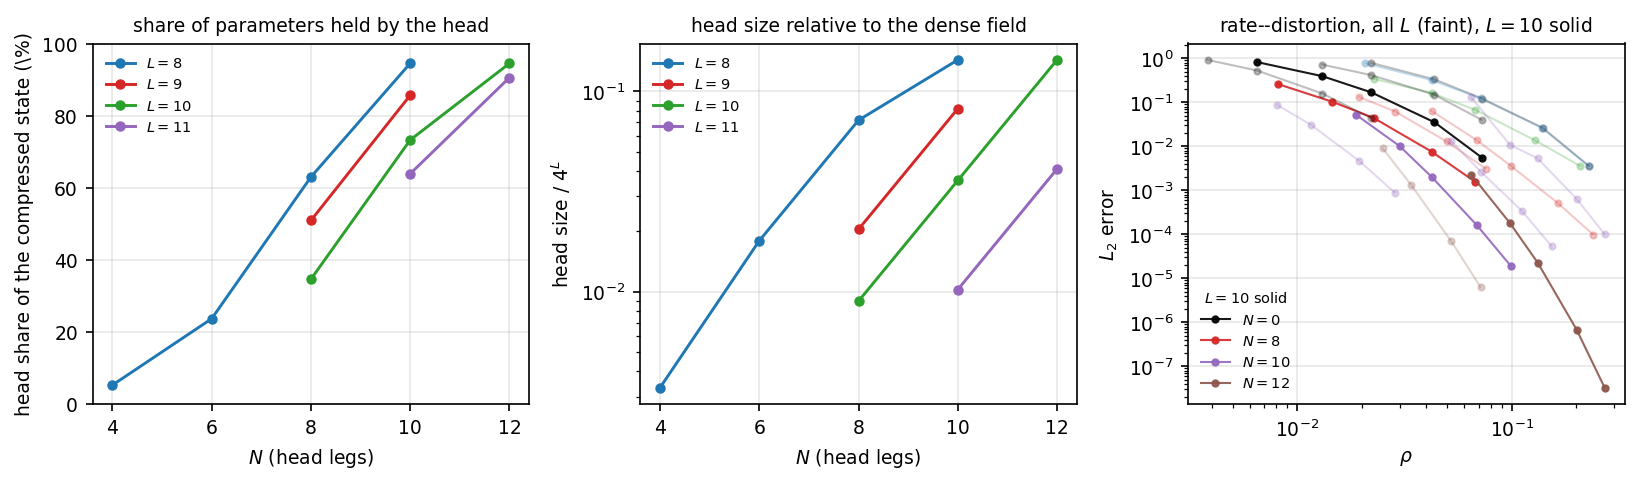
\includegraphics[width=\linewidth]{figures/head_budget.png}
\caption{Head cost under both normalisations, and the rate--distortion curves
from which the optimum is read. Left: share of the compressed state held by the
head. Centre: head size as a fraction of the dense field, which falls with $L$
at fixed $N-L$. Right: $L_2$ error against compression ratio $\rho$ for every
run; $L=10$ drawn solid.}
\label{fig:headbudget}
\end{figure}

\section{Rate--distortion}

Bond caps are integers, so the two encodings do not land on identical parameter
counts. Each encoding is therefore swept over bond caps and reported against the
compression ratio $\rho=\text{parameters}/4^L$ it achieves.
Table~\ref{tab:rd} lists every run. The reported error is the relative $L_2$
difference from a dense reference integrated with the same scheme, step and
velocity, averaged over the final third of the run, where it has saturated.

Alongside each evolution error is the error of compressing the \emph{exact}
field at the same budget, which separates the cost of representing the solution
from the additional cost of evolving in the representation.

\begin{table}[h]
\centering
\small
\TabRateDistortion
\caption{Every run. $N=0$ is the standard tensor train. ``head\,\%'' is the
share of the stored parameters occupied by the head.}
\label{tab:rd}
\end{table}

\section{Parameters required at fixed accuracy}

The quantity of practical interest is the budget required to reach a given
accuracy. Table~\ref{tab:saving} reports the ratio
$\rho_{\mathrm{std}}/\rho_{\mathrm{hybrid}}$, with the head size that achieves
the smaller budget, obtained by log--log interpolation of $\rho(\text{error})$.
Targets are listed only where both encodings span the target error.

\begin{table}[h]
\centering
\TabBudgetSaving
\caption{Parameters saved at fixed accuracy, and the head size achieving it.
The saving is $1.8$--$2.5$ and shows no trend with resolution over
$256^2$--$2048^2$.}
\label{tab:saving}
\end{table}

The error ratio read at fixed $\rho$ instead of fixed accuracy is considerably
larger --- at $L=10$ it runs from $2.8$ at $\rho=0.01$ to $25$ at $\rho=0.05$ ---
and it grows with resolution. Both quantities describe the same pair of curves.
The rate--distortion curves are steep and steepen with $L$, so a horizontal
offset of a factor $2$ in $\rho$ appears as one to two decades along the error
axis. The budget ratio is the quantity that answers how many parameters the head
buys.

\section{Evolution against representation}

Figure~\ref{fig:scaleup} collects the comparison across resolutions. The lower
middle panel plots the evolution error against the representation error at the
same budget for every run. All points lie between the $1\times$ and $25\times$
lines, with most below $5\times$, across four resolutions, five head sizes and
five bond caps.

The practical consequence is that the ordering of encodings in $N$ and the
scaling in $L$ can be established by compressing stored fields, which costs
minutes, rather than by integrating them, which costs core-days. The
representation measurement does not substitute for the evolution measurement
when the absolute error level matters.

\begin{figure}[h]
\centering
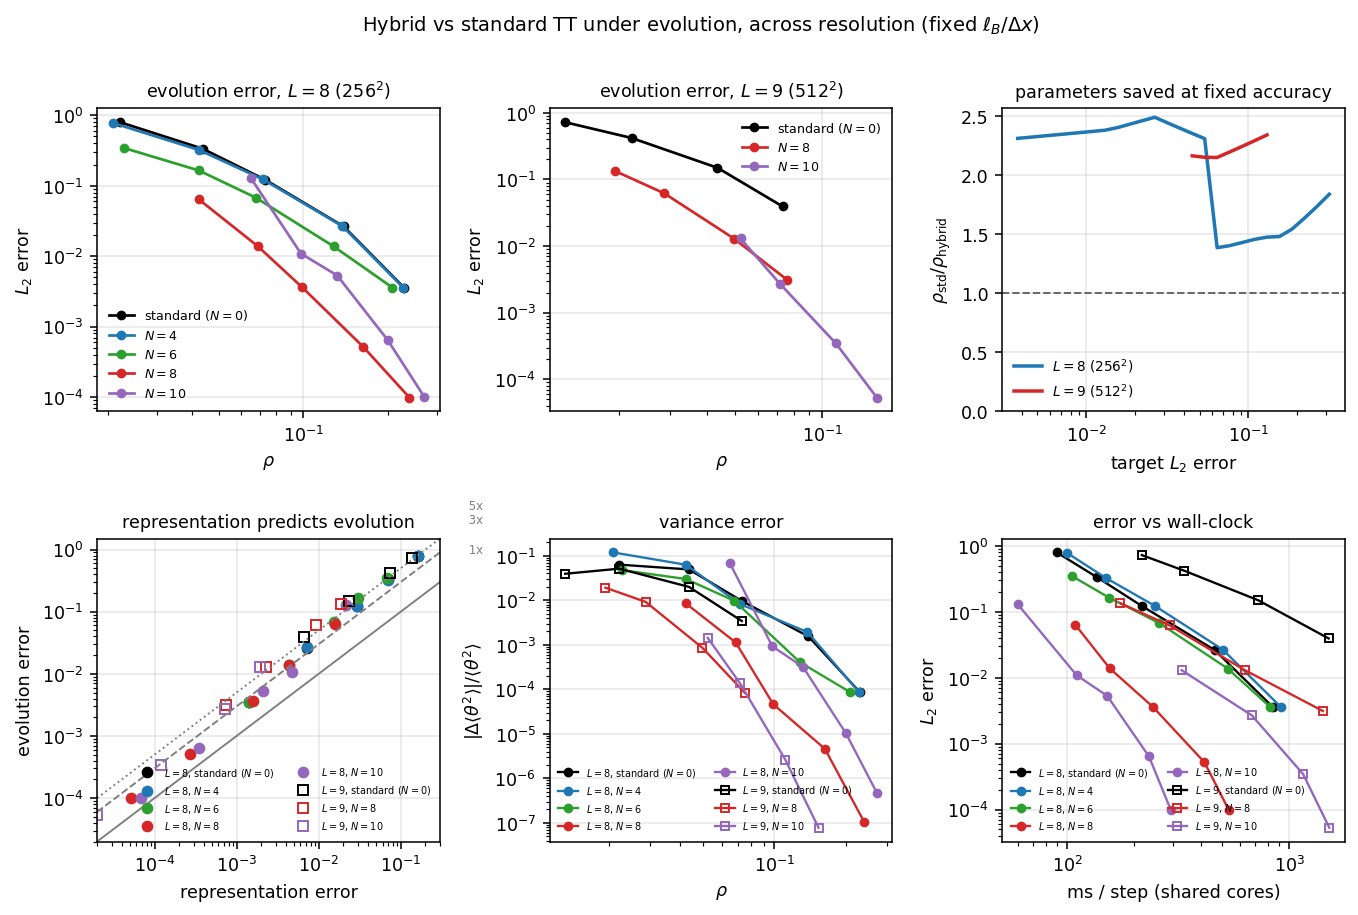
\includegraphics[width=\linewidth]{figures/scaleup_comparison.png}
\caption{Top: rate--distortion at $L=9,10,11$. Bottom left: parameters saved at
fixed accuracy. Bottom centre: evolution error against representation error at
the same budget, with $1\times$, $3\times$ and $5\times$ guides. Bottom right:
relative error in $\langle\theta^2\rangle$.}
\label{fig:scaleup}
\end{figure}

\section{Cost}

Table~\ref{tab:cost} gives measured cost per step at $\chi=32$. At equal bond
cap the hybrid encoding is slightly cheaper than the standard one, since it
carries $2L-N$ tail cores instead of $2L$, while the head contributes
$O(2^N r^2\chi)$ through the un-fusing path. At equal $\rho$ the comparison is
closer, because reaching a given $\rho$ with a larger head permits a smaller
$\chi$.

\begin{table}[h]
\centering
\TabCost
\caption{Measured cost per step at $\chi=32$. Runs shared cluster nodes, so
absolute values carry scheduling noise; the comparison within a row of constant
$L$ is the meaningful one.}
\label{tab:cost}
\end{table}

All runs are single-threaded. On a 256-core node, four threads instead of one
measured $29\times$ slower per step, because a step consists of thousands of
small contractions and SVDs, none large enough to amortise thread dispatch.

\section{Forced steady state}
\label{sec:forced}

The results above are obtained in a decaying cascade. To check that they are not
an artefact of the transient, the cellular flow was rerun at $256^2$ with a
steady source $f=0.8\sin 4y$ to $T=60$.

The forced wavenumber matters. The approach to a statistically steady state is
governed by the diffusive time of the forced scale, $1/(\kappa k_f^2)$, which is
$200$ time units at $k_f=1$; amplitudes from $0.02$ to $0.05$ were all still
climbing at $t=90$. At $k_f=4$ that time is $12$, and the variance plateaus by
$t\simeq40$, settling at $0.10$, $0.22$ and $0.51$ for amplitudes $0.3$, $0.5$
and $0.8$.

The forcing has zero box mean, so $\langle\theta\rangle$ is conserved: the
dense reference holds it to $3\times10^{-14}$ over $12\,222$ steps. Truncation
is not renormalised and no mass projection is applied, so the hybrid solver
instead drifts by an amount set by the budget, from $1.0\times10^{-2}$ at
$N=0$, $\chi=16$ to $1\times10^{-13}$ at $N=10$, $\chi=32$. The variance is
not conserved and is not expected to be: it rises to $1.51$ at $t\simeq4$ and
settles at $0.5109$, where production balances dissipation to $1.4\%$
($\langle\theta f\rangle=1.895\times10^{-2}$ against
$\kappa\langle|\nabla\theta|^2\rangle=1.922\times10^{-2}$ at $t=60$). What the
hybrid encoding reproduces is that steady level, to $3\times10^{-9}$ relative at
$N=8$, $\chi=32$.

In the steady state the variance holds to within $1.3\%$ beyond $t=36$, and the
intrinsic rank of the exact solution, probed at $\epsilon=10^{-6}$ in the $N=8$
layout, rises from $12$ to a peak of $56$ and settles at $41.7\pm0.5$ against a
geometric bound of $256$. The evolution error
is monotone in $\chi$ for every head size, and the budget saving over the
standard encoding is $1.4$ at $L_2=10^{-2}$, achieved at $N=6$
(Table~\ref{tab:forced}).

\begin{table}[h]
\centering
\small
\TabForced
\caption{Forced cellular flow, $256^2$, $f=0.8\sin 4y$, averaged over the final
third of the run.}
\label{tab:forced}
\end{table}

\begin{figure}[h]
\centering
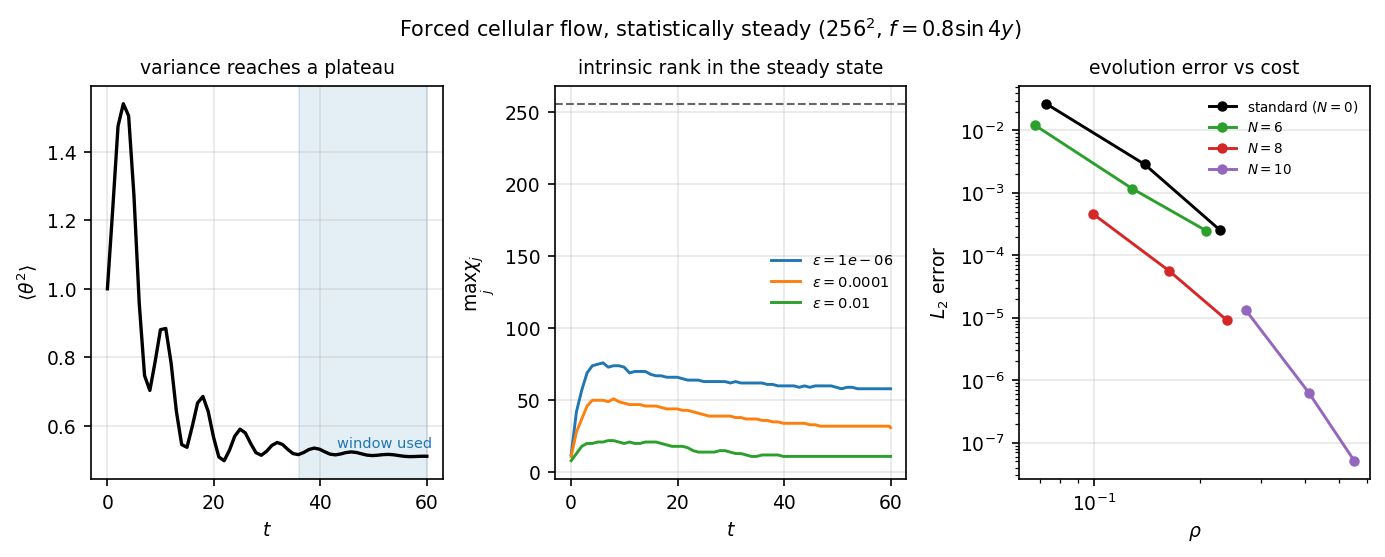
\includegraphics[width=\linewidth]{figures/forced_steady.png}
\caption{Variance plateau, intrinsic rank in the steady state, and
rate--distortion for the forced cellular flow.}
\label{fig:forced}
\end{figure}

\section{A frozen DNS velocity}
\label{sec:dns}

The cellular flow is integrable and its scalar spectrum steep, so the benchmark
was repeated with a velocity taken from the DNS dataset. The streamfunction was
recovered from the stored $v_x,v_y$ at $4096^2$ by inverting the vorticity
spectrally, coarsened to $512^2$, and differentiated with the solver's own MPOs,
leaving the velocity divergence-free to $2\times10^{-12}$ discretely.

The streamfunction itself is close to full rank. At $\epsilon=10^{-6}$ its bond
saturates the geometric bound and the tensor train costs more parameters than
the dense field, $\rho=1.33$ at $L=9$ and $2.32$ at $L=10$. It becomes
compressible only at $\epsilon=10^{-2}$, giving bond $21$ at $\rho=0.084$ for a
$1.7\%$ error in $\psi$. The runs therefore use a truncated velocity, carrying
$\chi(\mathbf{u})=34$ against $4$ for the cellular flow, at
$\rho(\mathbf{u})=0.14$, which makes a step about five times more expensive.
The measured strain rate is $\gamma=14.6$ and $u_{\max}=1.78$, so
$\kappa=1.5\times10^{-2}$ places the Batchelor scale at
$\ell_B/\Delta x=2.61$, close to the $2.88$ of the cellular ladder, and $T=2$
covers $29$ strain times.

The rank plateaus here as well, and faster: it is reached within a tenth of a
time unit and then holds at $315\pm1.1$ at $\epsilon=10^{-6}$ ($61\%$ of the
geometric bound), $154$ at $10^{-4}$ and $34$ at $10^{-2}$.

The evolution error, however, ceases to be monotone in the bond cap. At $N=10$
the $L_2$ error runs $7.7\times10^{-2}$, $1.5\times10^{-1}$,
$2.9\times10^{-2}$, $1.9\times10^{-3}$ for $\chi=16,24,32,48$, and the variance
error is non-monotone at $N=8$, $10$ and $12$. The representation error at the
same budgets is monotone in every case (Table~\ref{tab:dns}), which locates the
effect in the dynamics rather than in the encoding. The ratio of evolution to
representation error widens from $1.5$--$25$ for the cellular flow to
$1.5$--$233$ here.

Two consequences follow. The rate--distortion framing used above does not
transfer directly, since a given $(N,\chi)$ cannot be ranked by its budget
alone; and the budget saving can be quoted at only one accuracy target where the
two encodings overlap, $2.1$ at $L_2=10^{-1}$, achieved at $N=8$.

\begin{table}[h]
\centering
\small
\TabDNS
\caption{Frozen DNS velocity, $512^2$, $\psi$ truncated at $10^{-2}$, averaged
over the final third of the run.}
\label{tab:dns}
\end{table}

\begin{figure}[h]
\centering
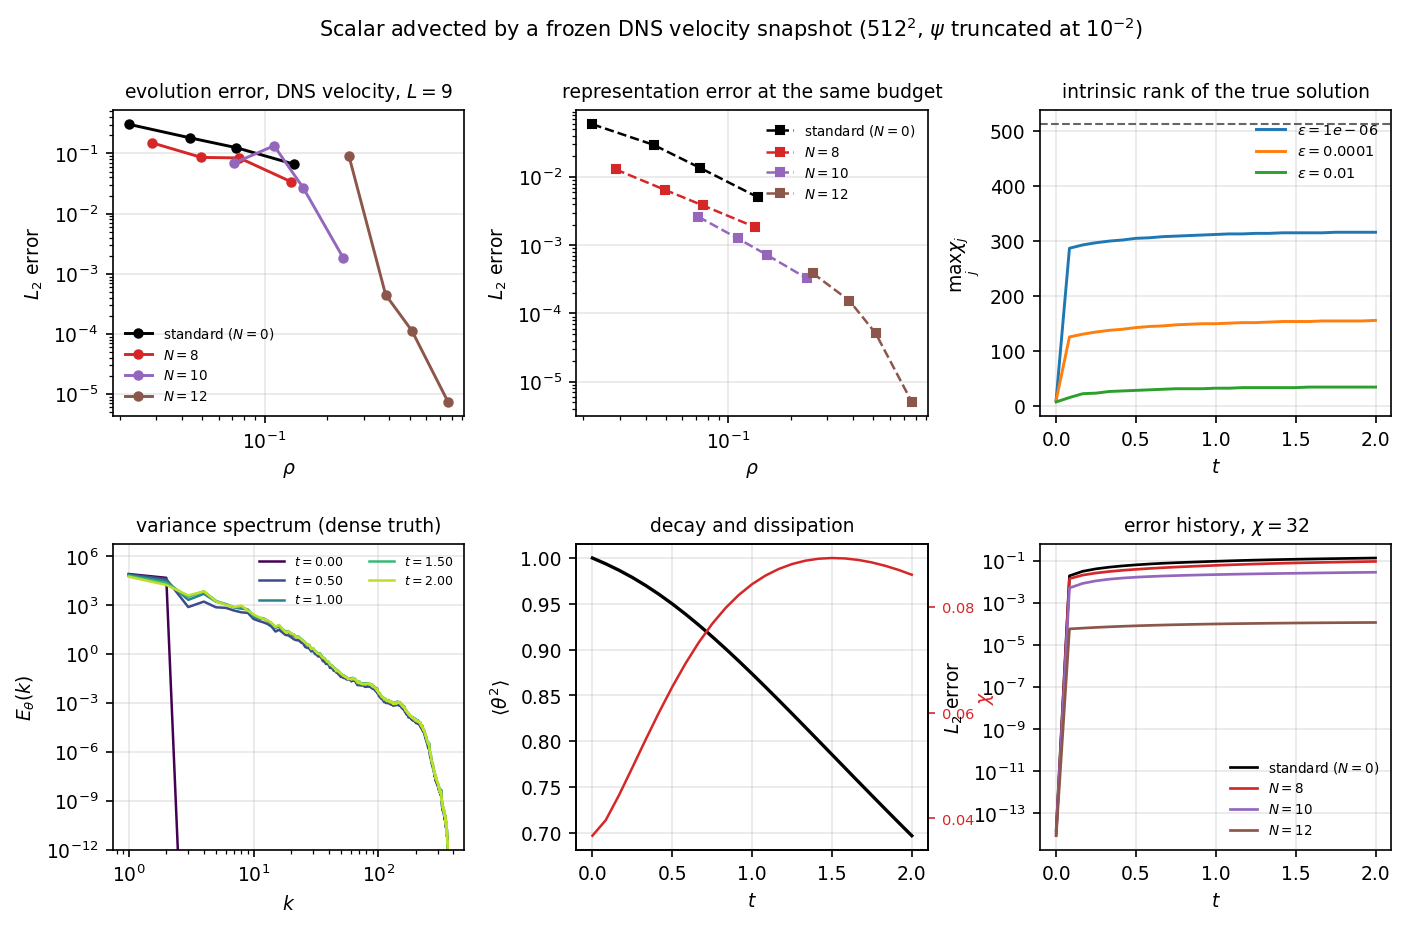
\includegraphics[width=\linewidth]{figures/dns_advection.png}
\caption{Scalar advected by a frozen DNS velocity snapshot: rate--distortion,
representation error at the same budgets, intrinsic rank, variance spectrum,
variance budget and error histories.}
\label{fig:dns}
\end{figure}

\section{Scope of these results}

The measurements above are specific to the flow used. The cellular flow
$\psi=\sin x\sin y$ has closed streamlines and is integrable, and its scalar
spectrum is steep, $E_\theta(k)\sim k^{-4.9}$ over $3\le k\le20$, rather than the
$k^{-1}$ Batchelor form of a chaotic flow. Breaking the streamlines with
$\psi=\sin(x+B\sin\omega t)\sin y$ raises the rank plateau from $75$ to $84$ at
$L=8$ and leaves the spectrum steep.

The size of the hybrid advantage depends on the field. On random-phase fields of
prescribed spectral slope the same measurement gives $1.2$ at $k^{-5/3}$ and
$3.5$ at $k^{-5}$, against $5$--$24$ at fixed $\rho$ for the cellular field. The
difference is attributable to spatial coherence rather than to spectral slope or
to alignment with the dyadic block boundaries: rigid shifts of the field by $2$,
$4$, $8$ and $13$ cells leave the advantage unchanged.

Real turbulent scalar fields lie between the two cases. The DNS-velocity run
above gives the first direct measurement on a realistic field: the advantage
persists, at $2.1$ in budget at $L_2=10^{-1}$, but the non-monotonicity of the
evolution error means a single number characterises it less completely than in
the cellular case. The representation measurements on DNS data reported in the
paper remain the reference point for the representation question.

One further check bears on those figures. \code{tt.svd} defaults to
\code{renormalize=True}, which rescales the kept singular values at every split.
On \code{theta.00059} at $4096^2$ the stored hybrid fields were found to equal
the plain rank-truncated field times a single global scalar $c$ to
$1.2$--$3.5\times10^{-14}$. The norm is preserved exactly, $E(1)$ shifts by
exactly $c^2$ --- $+2.7\%$ at $\rho=0.014$, falling to $+0.04\%$ at $\rho=0.64$
--- and the gradient flatness ratio is $1.0000$, so all scale-invariant
statistics are unaffected.

\section{Configuration}

\begin{itemize}
\item Grids $2^L\times2^L$ with $L=8,9,10,11$; $\kappa=5\times10^{-3}$,
  $1.25\times10^{-3}$, $3.125\times10^{-4}$, $7.8125\times10^{-5}$.
\item $\Delta t=0.2\,\Delta x$ (CFL-limited at every resolution), $T=8$, giving
  $1630$, $3259$, $6519$ and $13038$ steps.
\item Head sizes $N\in\{0,4,6,8,10,12\}$, bond caps $\chi\in\{4,\dots,64\}$
  applied uniformly as \code{bd\_first}~$=$~\code{bd\_remaining}, with
  \code{eps}~$=$~\code{None} (so the cap alone truncates $\theta$) and
  \code{renormalize}~$=$~\code{False} so that truncated norm is not restored.
\item $101$ production runs: $69$ cellular decaying ($29$ at $L=8$, $12$ at
  $L=9$, $20$ at $L=10$, $12$ at $L=11$), $12$ cellular forced and $16$ under
  the frozen DNS velocity. The $L=10$, $L=11$, forced and DNS sets were run as
  Slurm arrays, one core per task.
\end{itemize}

\end{document}
